
%%%%%%%%%%%%%%%%%%%%%%%%%%%%%%%%%%%%%%%%% 
% Beamer Presentation
% LaTeX Template
% Version 1.0 (10/11/12)
%
% This template has been downloaded from:
% http://www.LaTeXTemplates.com
%
% License:
% CC BY-NC-SA 3.0 (http://creativecommons.org/licenses/by-nc-sa/3.0/)
%
%%%%%%%%%%%%%%%%%%%%%%%%%%%%%%%%%%%%%%%%%

%----------------------------------------------------------------------------------------
%	PACKAGES AND THEMES
%----------------------------------------------------------------------------------------

\documentclass{beamer}

\mode<presentation> {

% The Beamer class comes with a number of default slide themes
% which change the colors and layouts of slides. Below this is a list
% of all the themes, uncomment each in turn to see what they look like.

%\usetheme{default}
%\usetheme{AnnArbor}
%\usetheme{Antibes}
%\usetheme{Bergen}
%\usetheme{Berkeley}
%\usetheme{Berlin}
%\usetheme{Boadilla}
\usetheme{CambridgeUS}
%\usetheme{Copenhagen}
%\usetheme{Darmstadt}
%\usetheme{Dresden}
%\usetheme{Frankfurt}
%\usetheme{Goettingen}
%\usetheme{Hannover}
%\usetheme{Ilmenau}
%\usetheme{JuanLesPins}
%\usetheme{Luebeck}
%\usetheme{Madrid}
%\usetheme{Malmoe}
%\usetheme{Marburg}
%\usetheme{Montpellier}
%\usetheme{PaloAlto}
%\usetheme{Pittsburgh}
%\usetheme{Rochester}
%\usetheme{Singapore}
%\usetheme{Szeged}
%\usetheme{Warsaw}

% As well as themes, the Beamer class has a number of color themes
% for any slide theme. Uncomment each of these in turn to see how it
% changes the colors of your current slide theme.

%\usecolortheme{albatross}
%\usecolortheme{beaver}
%\usecolortheme{beetle}
%\usecolortheme{crane}
%\usecolortheme{dolphin}
%\usecolortheme{dove}
%\usecolortheme{fly}
%\usecolortheme{lily}
%\usecolortheme{orchid}
%\usecolortheme{rose}
%\usecolortheme{seagull}
%\usecolortheme{seahorse}
%\usecolortheme{whale}
%\usecolortheme{wolverine}

%\setbeamertemplate{footline} % To remove the footer line in all slides uncomment this line
%\setbeamertemplate{footline}[page number] % To replace the footer line in all slides with a simple slide count uncomment this line

%\setbeamertemplate{navigation symbols}{} % To remove the navigation symbols from the bottom of all slides uncomment this line
}

\usepackage{graphicx} % Allows including images
\usepackage{booktabs} % Allows the use of \toprule, \midrule and \bottomrule in tables

\usepackage{bbm}
\usepackage{fixltx2e}
\usepackage{url}
\usepackage{amsmath, amsthm, amssymb}
\usepackage{mathtools}
\usepackage{multirow}
\usepackage{colortbl}
\usepackage{xspace}
\usepackage{verbatim}
\usepackage{graphicx}
\usepackage{psfrag}
\usepackage{natbib}
\usepackage{pbox}
\usepackage{epstopdf}
\usepackage{textcomp} % For copyright symbol
\DeclareGraphicsExtensions{.pdf,.eps,.png,.jpg}
\usepackage[font=singlespacing]{subcaption}
\captionsetup[table]{labelfont=bf,font=singlespacing}
\captionsetup[figure]{labelfont=bf,font=singlespacing}
\captionsetup[subfigure]{labelfont=bf,font=singlespacing}
\usepackage[titletoc,title]{appendix}
\usepackage{tabularx}
\usepackage{rotating}
\usepackage{hyperref} % Turns all internal references into links to pages within the document

\usepackage{lmodern} % Use the Latin Modern font
\usepackage[T1]{fontenc} % Use a modern font encoding

\newcommand{\Exp}[1]{\mbox{Exp}\left(#1\right)}
\newcommand{\Pois}[1]{\mbox{Pois}\left(#1\right)}

\newcommand{\hb}{\hat{b}}
\newcommand{\ha}{\hat{a}}
\newcommand{\htheta}{\hat{\theta}}
\newcommand{\halpha}{\hat{\alpha}}
\newcommand{\hmu}{\hat{\mu}}
\newcommand{\hsigma}{\hat{\sigma}}
\newcommand{\hphi}{\hat{\phi}}
\newcommand{\htau}{\hat{\tau}}
\newcommand{\heta}{\hat{\eta}}
\newcommand{\E}[1]{\mbox{E}\left[#1\right]}
\newcommand{\Var}[1]{\mbox{Var}\left[#1\right]}
\newcommand{\Indicator}[1]{\mathbbm{1}_{ \left( #1 \right) } }
\newcommand{\dNormal}[3]{ N\left( #1 \left| #2, #3 \right. \right) }
\newcommand{\Beta}[2]{\mbox{Beta}\left( #1, #2 \right)}
\newcommand{\alphaphi}{\alpha_{\hphi}}
\newcommand{\betaphi}{\beta_{\hphi}}
\newcommand{\expo}[1]{ \exp\left\{ #1 \right\}}
\newcommand{\tauSquareDelta}{\htau^2
  \left(\frac{1-\expo{-2\htheta\Delta}}{2\htheta} \right)}
\newcommand{\mumu}{\mu_{\hmu}}
\newcommand{\sigmamu}{\sigma^2_{\hmu}}
\newcommand{\sigmamuexpr}{\log\left( \frac{\VarX}{\EX^2} + 1 \right)}
\newcommand{\mumuexpr}{\log(\EX) -  \log\left( \frac{\VarX}{\EX^2} + 1 \right) /2 }

\newcommand{\EX}{\mbox{E}\left[ X \right] }
\newcommand{\VarX}{\mbox{Var}\left[ X \right] }
\newcommand{\mueta}{\mu_{\heta} }
\newcommand{\sigmaeta}{\sigma^2_{\heta}}
\newcommand{\sigmaetaexpr}{ \log\left( \frac{\VarX}{\EX^2} + 1 \right) }
\newcommand{\muetaexpr}{ \log(\EX) -  \sigmaetaexpr /2 }

\newcommand{\mualpha}{\mu_{\halpha} }
\newcommand{\sigmaalpha}{\sigma^2_{\halpha}}
\newcommand{\sigmaalphaexpr}{ \log\left( \frac{\VarX}{\EX^2} + 1 \right) }
\newcommand{\mualphaexpr}{ \log(\EX) -  \sigmaalphaexpr /2 }

\newcommand{\mutauexpr}{ \frac{2}{T} \EX }
\newcommand{\sigmatauexpr}{ \frac{4}{T^2} \Var{X}}

\newcommand{\alphatau}{\alpha_{\htau^2}}
\newcommand{\betatau}{\beta_{\htau^2}}

\newcommand{\Gam}[2]{\mbox{Gamma}\left( #1, #2 \right) }
\newcommand{\InvGam}[2]{\mbox{Inv-Gamma}\left( #1, #2 \right) }

%----------------------------------------------------------------------------------------
%	TITLE PAGE
%----------------------------------------------------------------------------------------

\title[]{Volatility and Correlation Analysis of Financial Market Data} % The short title appears at the bottom of every slide, the full title is only on the title page

\author{Georgi Dinolov} % Your name
\institute[UCSC] % Your institution as it will appear on the bottom of every slide, may be shorthand to save space
{
University of California, Santa Cruz \\ % Your institution for the title page
\medskip
\textit{gdinolov@soe.ucsc.edu} % Your email address
}
\date{\today} % Date, can be changed to a custom date

\begin{document}

\begin{frame}
\titlepage % Print the title page as the first slide
\end{frame}

\begin{frame}
\frametitle{Overview} % Table of contents slide, comment this block out to remove it
\tableofcontents % Throughout your presentation, if you choose to use \section{} and \subsection{} commands, these will automatically be printed on this slide as an overview of your presentation
\end{frame}

%----------------------------------------------------------------------------------------
%	PRESENTATION SLIDES
%----------------------------------------------------------------------------------------

%------------------------------------------------
\section{Introduction}
%------------------------------------------------

\begin{frame}
\frametitle{Two Data Types: High-Frequency and Open, Close High, Low Prices}
\begin{itemize}
  \item high-frequency prices
  \item open, close, high, low as summaries of volatility
\end{itemize}
\end{frame}

%------------------------------------------------
%------------------------------------------------
\section{High-Frequency Prices}
%------------------------------------------------
\begin{frame}
  \frametitle{High-frequency returns and difficulties}
  \begin{itemize}
  \item As sampling frequency approaches transaction-by-transaction
    frequency, \textbf{irregular spacing} between transactions, \textbf{discreteness} in
    transaction prices (such as the bid-ask spread), and very short term \textbf{temporal dependence} become
    dominant features of the data \citep{stoll2000presidential}.

  \item These confounding effects in estimating volatility are
    generally termed \textbf{microstructure noise}.

    \begin{itemize}
    \item independent of sampling interval,
    \item dominant over short time ($<5$ minutes),
    \item not cumulative (prices at later times are not affected)
    \end{itemize}

  \end{itemize}
\end{frame}
% ------------------------------------------------
\begin{frame}
  \frametitle{Past work and model-bashed incoherence}
  \begin{itemize}
  \item Attempts have been made to fit the GARCH model to
    high-frequency data \citep{bollerslev1986,andersen1997intraday}.

  \item As formulated, such types of models are are not
    robust with respect to the specification of the sampling interval
    \citep{drost1993aggregation, andersen1997intraday,
      zumbach2000pitfalls}.

  \item Inference over shrinking sampling intervals leads to
    \textbf{incoherence}.

  \item Most recent work has forcused on the \textbf{realized variance} estimator:
    \[
      RV_T := \sum_{i=1}^{N/\Delta t} r_{t_i}^2,
    \]
    where $r_{t_i}^2$ is the squared \textit{return} observed over $[t_{i-1}, t_i]$.
  \end{itemize}
\end{frame}
% ------------------------------------------------
\begin{frame}
  \frametitle{Realized variance estimator}
  In the absence of microstructure noise, 
  \[
    RV_t = \sum_{i=1}^{N/\Delta t} r_{t_i}^2 \,\,\, \to \,\,\, \displaystyle \int_{0}^T \sigma^2\left(X_t, t\right)\, dt
  \]
  
  \begin{itemize}
  \item Corrections for the presence of microstructure noise have been
    successfully proposed in the form of:
    \begin{itemize}
    \item sampling sparser grids and averaging,
    \item combining estimators based on subsampled data at different frequencies,
    \item kernel-based estimation.
    \end{itemize}
  \item Disadvantages: averages out information; no inherent
    model-based projection forward in time.
  \end{itemize}
\end{frame}
% ------------------------------------------------
\begin{frame}
  \frametitle{A filtering-based approach} Given the \textbf{true}
  price $S_j$ at sample index $j$, we model the \textbf{measured} price $P_j$ as contaminated by noise due to the bid-ask spread $D$:
  \begin{align*}
    P_j &= S_j + \nu_j,& \nu_j &\sim U[-D/2, D/2],
  \end{align*}

  A first-order Taylor expansion of the \textbf{observed log price} $\log(P_j)$ produces
  \begin{align*}
    log(P_j) &\approx log(S_j) + \frac{1}{S_j}\nu_j.
  \end{align*}

  We further model the noise term with a Gaussian distribution
  \begin{align*}
    \zeta_j := \frac{1}{S_j}\nu_j \sim N\left(0, \frac{D}{4Q^2} \right)
  \end{align*}
  where $Q$ is an order-magnitude approximation of the true price
  $S_j$.
\end{frame}
% ------------------------------------------------
\begin{frame}
  \frametitle{Full \textit{continuous-time} formulation} We represent
  the idealized joint log-price $\log(\hat{S}_t)$ and log-volatility
  $\log(\hat{\sigma}_{t,1}), \log(\hat{\sigma}_{t,2})$ diffusion
  process as the system of SDEs:
  \begin{align*}
  d\log(\hat{S}_t) &= \hat{\mu}\, dt + \sqrt{\hat{\sigma}_{t,1} \hat{\sigma}_{t,2}}\, \sqrt{dt} \hat{\epsilon}_{t} + dJ_t  ,   \\
  d\log( \hat{ \sigma }_{t,1}) &= -\hat{\theta}_1 ( \log(\hat{\sigma}_{t,1} ) - \hat{\alpha} )\, dt + \hat{\tau}_1\, \sqrt{dt} \hat{\epsilon}_{t,1}  , \\
  d\log( \hat{ \sigma }_{t,2}) &= -\hat{\theta}_2 ( \log(\hat{\sigma}_{t,2} ) - \hat{\alpha} )\, dt + \hat{\tau}_2\, \sqrt{dt} \hat{\epsilon}_{t,2}  . 
  \end{align*}

  \begin{itemize}
  \item $\log(\hat{\sigma}_{t,1})$ evolves stochastically with long time scale $1/\hat{\theta}_1,$
  \item $\log(\hat{\sigma}_{t,2})$ evolves stochastically with short time scale $1/\hat{\theta}_2,$
  \item $dJ_t$ is a compound Poisson process,
  \item $\hat{\epsilon}_t, \hat{\epsilon}_{t,1}, \hat{\epsilon}_{t,2}$ are Wiener processes with 
    \begin{align*}
      \E{\hat{\epsilon}_t\hat{\epsilon}_{t,2}} &= \rho, & \E{\hat{\epsilon}_t\hat{\epsilon}_{t,2}} &= 0, & \E{\hat{\epsilon}_{t,1}\hat{\epsilon}_{t,2}} &= 0.
    \end{align*}
  \end{itemize}
    
\end{frame}
% ------------------------------------------------
\begin{frame}
  \frametitle{Discrete interpretation of the formulation}
  Defining the log of the observed price $P_j$ as $Y_j := \log(P_j)$
  \begin{align*}
    Y_j &= \log(S_j) + \zeta_j  ,\\
    \log(S_{j}) &= \log(S_{j-1}) + \mu(\Delta) + \sqrt{\sigma_{j,1}\sigma_{j,2}} \, \epsilon_{j} + J_j(\Delta)   ,  \\
    \log(\sigma_{j+1,1}) &= \alpha(\Delta) + \theta_1(\Delta) \left\{ \log(\sigma_{j,1}) - \alpha(\Delta) \right\} + \tau_1(\Delta) \, \epsilon_{j,1}    ,  \\
    \log(\sigma_{j+1,2}) &= \alpha(\Delta) + \theta_2(\Delta) \left\{ \log(\sigma_{j,2}) - \alpha(\Delta) \right\} + \tau_2(\Delta) \, \epsilon_{j,2}.
  \end{align*}

  \begin{align*}
  \sigma_{j+1,i} &= \hat{\sigma}_{(j+1)\Delta,i}\sqrt{\Delta}, & S_j &= \hat{S}_{j\Delta}, & J_j(\Delta) &= J((j+1)\Delta) - J(j\Delta)
  \end{align*}
  
\begin{align*}
  \begin{split}
    \alpha(\Delta) = \halpha + \frac{1}{2}\log(\Delta),\quad  & 
    \mu(\Delta) = \hat{\mu} \Delta,      \\
    \tau_i(\Delta) = \hat{\tau}_i \sqrt{ \frac{1 - \exp \left\{
          -2\hat{\theta}_i \Delta \right\}}{2\hat{\theta}_i } },\quad & \theta_i(\Delta) =
    \exp\left\{
      -\hat{\theta}_i \Delta \right\}.
    \end{split}
\end{align*}
\end{frame}
% ------------------------------------------------
\begin{frame}
  \frametitle{Prior formulation} To ensure that the model estimation
  is coherent across choices of sampling periods $\Delta$, we
  
  \begin{enumerate}
  \item define the first two moments of each continuous-time parameter,
  \item define the prior for each continuous-time parameter,
  \item use the Delta Method to calculate the first two moments of each discrete-time parameter,
  \item define the prior for each discrete-time parameter.
  \end{enumerate}

  Example:
  \begin{align}
    \tau^2(\Delta) &\sim \mbox{Inv-Gamma}\left(  a_{\tau^2}(\Delta), b_{\tau^2}(\Delta) \right) \\
    \mbox{E}(\tau^2(\Delta)) &\approx f(a_{\hat{\tau}^2}, b^2_{\hat{\tau}^2}, \Delta) \\
    \mbox{Var}(\tau^2(\Delta)) &\approx g(a_{\hat{\tau}^2}, b^2_{\hat{\tau}^2}, \Delta)
  \end{align}
\end{frame}
% ------------------------------------------------
\begin{frame}
  \frametitle{Computation}
  \begin{itemize}
  \item We separate the standard innovation term from volatility
    factors $\sigma_{j,1}$ and $\sigma_{j,2}$ by considering the
    transformation
  \begin{multline*}
    \log(S_{j}) = \log(S_{j-1}) + \mu(\Delta) + \sqrt{\sigma_{j,1}\sigma_{j,2}} \, \epsilon_{j} + J_j(\Delta) \\
  \leftrightarrow \quad \underbrace{ \log\left[ \left| \log(S_{j}/S_{j-1}) - \mu(\Delta) - J_j(\Delta) \right| \right] }_{y_j^*} = \frac{1}{2}\underbrace{  \log(\sigma_{j,1}) }_{h_{j,1}} + \frac{1}{2}\underbrace{  \log(\sigma_{j,2}) }_{h_{j,2}} \\
   + \underbrace{ \log(  \epsilon_{j}^2  )/2 }_{\epsilon_{j}^{*}}.
 \end{multline*}
 \pause
\item We approximate $\epsilon^*_{j}$ as a mixture of Normals
 \[
   \epsilon^*_{j} = \log( \epsilon_{j}^2 )/2 \sim \sum_{l=1}^{10} p_l N \left( \frac{m_l}{2}, \frac{v_l^2}{4} \right).
 \]
\end{itemize}
\end{frame}
% ------------------------------------------------
\begin{frame}
  \frametitle{Computation, continued}
  The joint distribution $(\epsilon^*_j, \epsilon_{j,2})$ conditional on the latent mixture element $\gamma_j$ becomes
  \begin{align*}
    p(\epsilon^*_j, \epsilon_{j,2} | \gamma_j) &= p(\epsilon_{j,2}|\epsilon^*_{j}, \gamma_j)p(\epsilon^*_{j}| \gamma_j) \\
                                               &= p(\epsilon_{j,2}|\underbrace{d_j exp(\epsilon^*_{j})}_{\epsilon_j}, \gamma_j)p(\epsilon^*_{j}| \gamma_j) \\
    &= N\left( \epsilon_{j,2} \left| d_j exp(\epsilon^*_{j}), (1-\rho^2) \right.\right) N\left( \epsilon_j^* \left| \frac{m_{\gamma_j}}{2}, \frac{v^2_{\gamma_j}}{4} \right. \right),
  \end{align*}
  where $d_j$ is the sign of $\epsilon_j$. \pause The joint
  distribution becomes a linear combination of independent Normal
  random variables when we replace the nonlinear $exp(\epsilon^*_{j})$
  term with the first-order Taylor expansion
  \[
    exp(\epsilon^*_{j}) | \gamma_j \approx \exp(m_{\gamma_j}/2)(a_{\gamma_j} + b_{\gamma_j}(2\epsilon_j^* - m_{\gamma_j}))
  \]
 
\end{frame}
% ------------------------------------------------
\begin{frame}
  \frametitle{Blocked Gibbs sampler with MH steps}
  \begin{enumerate}
  \item sample observational parameters
  \item sample latent prices
  \item sample volatility parameters
  \item sample latent mixture indicators
  \item sample valatility paths
  \item sample jump parameters
  \item sample jumps
  \end{enumerate}
\end{frame}
% ------------------------------------------------
\begin{frame}
  \frametitle{Estimating integrated volatility}
  \begin{itemize}
    \item We consider 300 simulated data sets over 1 trading day
  
    \item Percentage of $95\%$ probability/confidence intervals
      cover the true data-generating integrated volatility
      $\int \hat{\sigma}_t dt$:
  \end{itemize}
  \begin{table}[h]
\begin{center}
  \begin{tabular}{|l|ccccc|}
    \hline
    & \multicolumn{4}{c|}{Sampling period} \\
    &   	60 sec 	&   30 sec   &   15 sec & 5 sec  \\ \hline \hline
    Inference with $\xi^2 = 0$   &  72  &   28  &	 3 & 0 \\
    Inference with $\xi^2$ fixed at prior mean &  79 & 57 & 23 & 0 \\
    Inference with $\xi^2$ estimated & 91 & 92 & 96 & 97  \\ \hline
    Inference with kernel-based estimator &  51 & 48 & 59  & 76 \\
    \hline
\end{tabular}
\end{center}
\end{table}
\end{frame}
% ------------------------------------------------
\begin{frame}
  \frametitle{Parameter results for real data example}
\end{frame}

%------------------------------------------------
%------------------------------------------------
\section{Open, Close, High, Low Prices}
%------------------------------------------------
\begin{frame}
  \frametitle{Open, Close, High, Low Prices}
  Previous work, absence of bivariate solution
\end{frame}
% ------------------------------------------------
\begin{frame}
  \frametitle{Model formulation}
  We consider a two-dimensional correlated Brownian motion:
\begin{align}
  X(t) &= x_0 + \mu_x t + \sigma_x W_x(t)  \label{eq:X} \\
  Y(t) &= y_0 + \mu_y t + \sigma_y W_y(t)  \label{eq:Y}
\end{align}
where $W_x(t)$ and $W_y(t)$ are correlated standard Brownian motions
with $\mbox{Cov}(W_x(t), W_x(t)) = \rho t$.

\begin{itemize}
\item We seek the 6-dimensional joint probability density
function for the pair $(X(t), Y(t))$ and the random variables
$M_X(t)=\max_{0\leq s\leq t}X(s),$ $m_X(t)=\min_{0\leq s\leq t}X(s),$
$M_Y(t)=\max_{0\leq s\leq t}Y(s),$ $m_Y(t)=\min_{0\leq s\leq t}Y(s)$.
\end{itemize}
\end{frame}
% ------------------------------------------------
\begin{frame}
  \frametitle{Transition density} To calculate the joint density
  \begin{multline*}
    p(X(t) = x, Y(t) = y, \\
    m_X(t) = a_x, M_X(t) = b_X, m_Y(t) = a_Y, M_Y(t) = b_Y),
  \end{multline*}
  we first study cumulative-like distribution
  \begin{multline*}
    p(X(t) = x, Y(t) = y, \\
    m_X(t) \geq a_x, M_X(t) \leq b_X, m_Y(t) \geq
    a_Y, M_Y(t) \leq b_Y),
  \end{multline*}
  which is governed by a Fokker-Planck equation with absorbing boundaries:
\end{frame}
% ------------------------------------------------
\begin{frame}
  \frametitle{Governing Fokker-Planck equation}
  Abbreviating 
  \begin{multline*}
    q(x,y,t) := p(X(t) = x, Y(t) = y, \\
    m_X(t) \geq a_x, M_X(t) \leq b_X, m_Y(t) \geq
    a_Y, M_Y(t) \leq b_Y),
  \end{multline*}
  the FP equation is
  \begin{multline*}
    \displaystyle \frac{\partial}{\partial t'} q(x,y,t') = -\mu_x \frac{\partial}{\partial x}q(x,y,t')
    - \mu_y \frac{\partial}{\partial y}q(x,y,t') + \\
    \frac{1}{2}\sigma_x^2 \frac{\partial^2}{\partial x^2}q(x,y,t') + \rho\sigma_x\sigma_y \frac{\partial^2}{\partial x \partial y}q(x,y,t')
    + \frac{1}{2}\sigma_y^2 \frac{\partial^2}{\partial y^2}q(x,y,t'),
  \end{multline*}
  \begin{align*}
    q(a_x, y,t') &= q(b_x,y,t') = q(x,a_y,t') = q(x,b_y,t') = 0, & 0 &< t' \leq t, \\
    q(x,y,0) &= \delta(x_0 - x)\delta(y_0 - y)
  \end{align*}

\end{frame}
% ------------------------------------------------
\begin{frame}
  \frametitle{Normalized problem}
  We can introduce a series of transformations to solve the equivalent initial-boundary problem
  \begin{align*}
    \frac{\partial}{\partial \tilde{t}} q(\tilde{x},\tilde{y},\tilde{t}) &= \tilde{\mathcal{L}} q(\tilde{x},\tilde{y},\tilde{y}), & (\tilde{x}, \tilde{y}) \in \tilde{\Omega} \\
    \tilde{\mathcal{L}} &= \frac{1}{2} \frac{\partial^2}{\partial \tilde{x}^2} + \rho \sigma_{\tilde{y}} \frac{\partial^2}{\partial \tilde{x} \partial \tilde{y}} + \frac{1}{2} \sigma^2_{\tilde{y}} \frac{\partial^2}{\partial \tilde{y}^2},& \tilde{\Omega} := (0,1) \times (0,1)
  \end{align*}
  where $0 < \sigma_{\tilde{y}}^2 \leq 1$, and the terminal time
  $\tilde{T}$ at which we need to evaluate the transition density is
  bounded below by $0$.

  \begin{itemize}
  \item This new parameterization makes the computational domain invariant
  to data/parameter combinations.
  \end{itemize}
\end{frame}
% ------------------------------------------------
\begin{frame}
  \frametitle{Joint density is given by the fourth derivative with respect to boundaries}
  Denoting the joint density of the diffusion process and the attained extrema over the interval $t$ as
  $f(x,y,a_x,b_x,a_y,b_y)$,
  \begin{align*}
  \frac{\partial^4}{\partial a_x \partial b_x \partial a_y \partial b_y} q(x,y,t) = f(x,y,a_x,b_x,a_y,b_y).
  \end{align*}

  \begin{itemize}
  \item The finite difference approximation of
    $\partial^4/\partial a_x \partial b_x \partial a_y \partial b_y$
    introduces a fundamental limitation due to finite precision
    round-off errors when the analytic solution $q(x,y,t)$ is not available
    \[
      \mathcal{O}\left(\frac{\varepsilon_{mach}}{\varepsilon^4} \right) \to \infty \,\,\, \mbox{ as } \,\,\, \varepsilon \to 0,
    \]
    where $\varepsilon$ is the step size with respect to the boundaries.
  \end{itemize}
\end{frame}
% ------------------------------------------------

\begin{frame}
  \frametitle{Approach 1: Finite Difference}
  Requires the solution to a system of ODEs:
  \begin{align*}
    & \dot{c}(\tilde{t}) = Bc(\tilde{t}) &\Rightarrow& c(\tilde{t}) = \exp\left(B\tilde{t}\right)c(0), 
  \end{align*}
  where the sparse system matrix $B$ can be computed once and stored for a regular grid over $\tilde{\Omega}$ with finite step size $h$. 
  \[ B = \frac{1}{2} \frac{1}{h^2}B_{\tilde{x},\tilde{x}} +
    \rho\sigma_{\tilde{y}} \frac{1}{4h^2}B_{\tilde{x},\tilde{y}} +
    \frac{1}{2}\sigma_{\tilde{y}}^2
    \frac{1}{h^2}B_{\tilde{y},\tilde{y}}.
\]
\end{frame}
% ------------------------------------------------
\begin{frame}
  \frametitle{Approach 1: Finite Difference}
  Letting $k := 1/h$ and $b$ denote the boundary parameters, 
\begin{itemize}
  \item FD approximation is fast but also limited by irregular truncation errors
  \begin{multline*}
    q^{(k)}(\tilde{x},\tilde{y},\tilde{t} | b) - q(\tilde{x},\tilde{y},\tilde{t} | b) = \underbrace{\left( \frac{1}{k}
    \right)^{\alpha} \mbox{F}_{reg}(b)}_{\mbox{smooth in } b, \,\,\alpha > 0} \\
    + \underbrace{\left( \frac{1}{k}\right)^{\beta}\mbox{F}_{irreg}(b)}_{\mbox{continuous but not differentiable w.r.t }b, \,\, \beta > 0} + \underbrace{\varepsilon_{mach}F_{round}(b)}_{\mbox{behaves as a R.V}}
  \end{multline*}
  \item With linear interpolation which arises when function arguments are not on grid points
  \begin{align*}
    \mathcal{O}(F_{irreg}(b)) &= k^\beta/\varepsilon &\Rightarrow \left( \frac{1}{k}\right)^{\beta}\mbox{F}_{irreg}(b) &\to \infty \,\,\, \mbox{as} \,\,\, \varepsilon \to 0.
  \end{align*}
\end{itemize}
\end{frame}
% ------------------------------------------------
\begin{frame}
  \frametitle{Approach 2: Trigonometric expansion}
  \begin{align*}
    q(\tilde{x},\tilde{y},\tilde{t}) &\approx  \sum_\nu h_\nu \phi_\nu (\tilde{x}, \tilde{y}) e^{-\lambda_\nu \tilde{t}}, \\
    \phi_\nu(\tilde{x},\tilde{y}) &= \sum_{l=1}^L \sum_{m=1}^M c_{l,m, \nu}
                                    \sin\left(2\pi\, l\, \tilde{x} \right) \sin\left(2\pi\, m\, \tilde{y} \right) := \Psi(\tilde{x},\tilde{y})^T c_\nu, \\
    \mathcal{L}\phi_\nu &= \mathcal{L}(\Psi(\tilde{x},\tilde{y})^T c_\nu) =
  \mathcal{L}(\Psi(\tilde{x},\tilde{y})^T) c_\nu = (A \Psi(\tilde{x},\tilde{y}))^T c_\nu = -\lambda_\nu \phi_\nu
  \end{align*}
  \begin{itemize}
  \item When $\rho = 0$,
    \begin{itemize}
    \item the system matrix $A$ is diagonal,
    \item no new error is introduced in the time evolution,
    \item truncated solution converges fast
    \end{itemize}
  \item When $\rho \neq 0$, mixing term in the FP equation produces
    $\cos(2\pi l \tilde{x})\cos(2\pi k \tilde{y})$ terms such that
    \begin{itemize}
    \item $A$ is dense and convergence is slow,
    \item new error is introduced in the time evolution
    \end{itemize}
  \end{itemize}
\end{frame}
% ------------------------------------------------

\begin{frame}
  \frametitle{The Galerkin approach: weak solution to the PDE}
  We propose a solution $q^{(k)}(\tilde{x},\tilde{y},\tilde{t})$ of similar
  form
  \[
    q^{(k)}(\tilde{x},\tilde{y},\tilde{t}) = \sum_{i=0}^k c_i(\tilde{t})
    \psi_i(\tilde{x},\tilde{y}),
  \]
  where the basis functions $\psi_i(\tilde{x},\tilde{y})$ satisfy the
  boundary conditions on $\tilde{\Omega}$. We also require that all
  first- and second-order derivatives of $\psi_i(\tilde{x},\tilde{y})$
  are in $L_2(\tilde{\Omega})$.
  \begin{align*}
  \frac{\partial}{\partial \tilde{t}} q^{(k)}(\tilde{x},\tilde{y},\tilde{t}) - \tilde{\mathcal{L}}q^{(k)}(\tilde{x},\tilde{y},\tilde{t}) &:= R_e(k), \\
  q(\tilde{x},\tilde{y},0) - q^{(k)}(\tilde{x},\tilde{y},0) &:= R_0(k).
  \end{align*}
\end{frame}
% ------------------------------------------------
\begin{frame}
  \frametitle{The Galerkin approach: weak solution to the PDE}
  The \textit{orthogonality} condition coincides with the
  Galerkin procedure:
  \begin{align*}
    \displaystyle \int_{\Omega} R_e(k) \psi_i(\tilde{x},\tilde{y}) d\tilde{x}\,d\tilde{y} &= 0,& \displaystyle \int_{\Omega} R_0(k) \psi_i(\tilde{x},\tilde{y}) d\tilde{x}\,d\tilde{y} &= 0,& i = 0,\ldots k, 
  \end{align*}
  which is equivalent to the weak formulation of the heat problem
  \begin{align*}
    \left< \partial_t q^{(k)}(\tilde{x},\tilde{y},\tilde{t}), \psi_i \right> &= \left<\tilde{\mathcal{L}}q^{(k)}(\tilde{x},\tilde{y},\tilde{t}), \psi_i \right>, \\
    \left< q^{(k)}(\tilde{x},\tilde{y},0), \psi_i \right> &= \left<q(\tilde{x},\tilde{y},0), \psi_i\right>,
  \end{align*}
  where $<\cdot, \cdot>$ is the usual inner product in
  $L_2(\tilde{\Omega})$.
\end{frame}
% ------------------------------------------------
\begin{frame}
  \frametitle{Basis element choice}
  \begin{align*}
    \psi_i(\tilde{x},\tilde{y}) &= \frac{1}{2\pi \tilde{\sigma}^2\sqrt{1-\tilde{\rho}^2} } \\
                                &\quad \times \exp\left\{ -\frac{\left( (\tilde{x} - \tilde{x}_i)^2 - 2\tilde{\rho} (\tilde{x}-\tilde{x}_i)(\tilde{y}-\tilde{y}_i) + (\tilde{y} - \tilde{y}_i)^2 \right)}{2(1-\tilde{\rho}^2)\tilde{\sigma}^2}  \right\} \nonumber \\
                                &\quad \times \tilde{x}\left(1-\tilde{x}\right)\, \tilde{y}(1-\tilde{y}) \nonumber
  \end{align*}
  for some parameters $(\tilde{\rho}, \tilde{\sigma})$ and a collection of nodes
  $\{ (\tilde{x}_i,\tilde{y}_i) \}_{i=0}^k$ which form a grid over
  $\tilde{\Omega}$.
  \begin{itemize}
  \item Align basis elements along the principal axis of the differential operator,
  \item Spacing between nodes is $l$ times the bandwidth $\tilde{\sigma}$ in each principal direction
  \item This scheme is aimed at better resolving the initial condition (elaborated below)
  \end{itemize}
\end{frame}
% ------------------------------------------------
\begin{frame}
\begin{figure}
  \centering
  %%
  %%
  \begin{tabular}{cc}
    \begin{minipage}{0.4\textwidth}
      \centering
      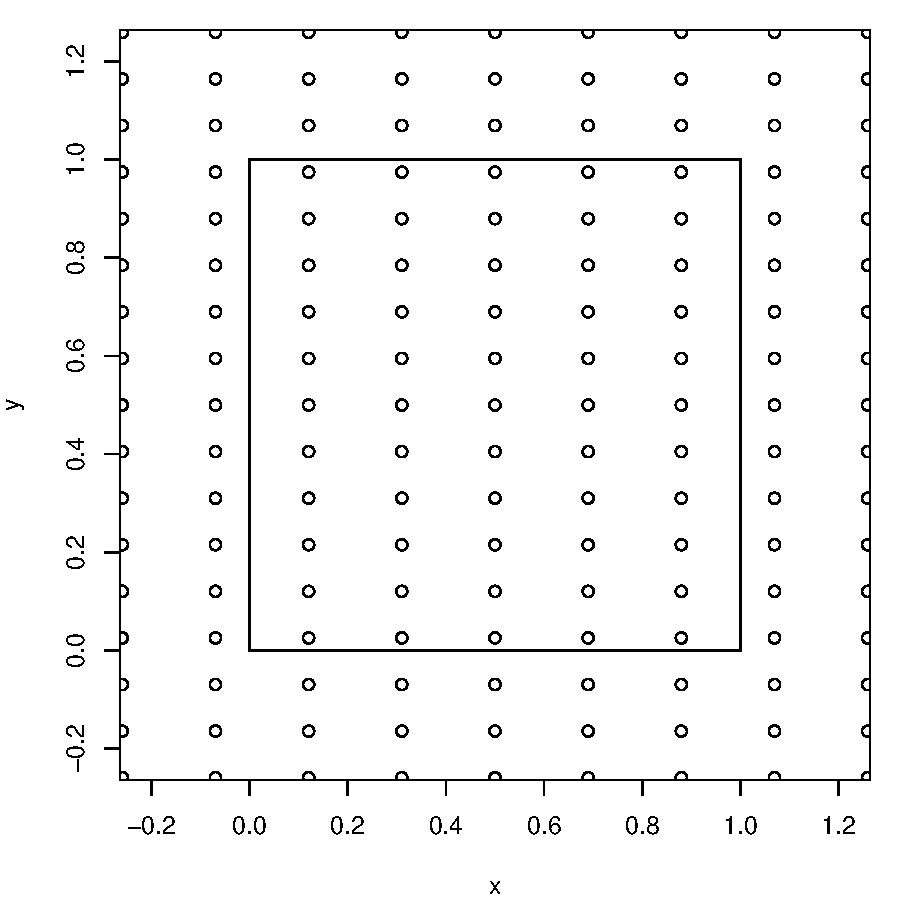
\includegraphics[width=1\linewidth]{../nodes-1.pdf}
    \end{minipage}
    %%
    & \begin{minipage}{0.4\textwidth}
      \centering
      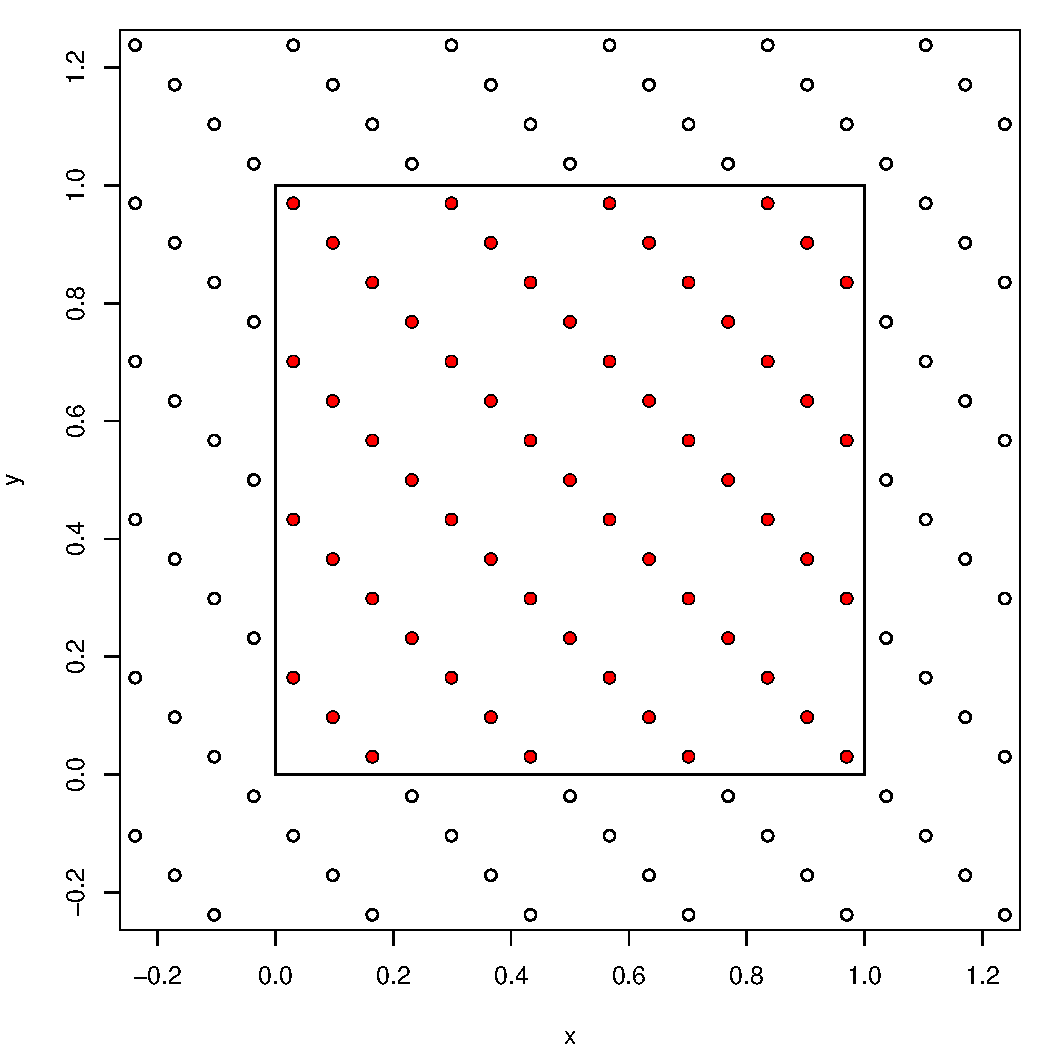
\includegraphics[width=1\linewidth]{../nodes-2.pdf}
    \end{minipage}
  \end{tabular}
  %%
  %%
  % \caption{A sample grid design for $l=1$, $\sigma=0.3$ and $\rho=0.6$. The
  %   left panel corresponds to the initial grid
  %   $\{ (x'_j,y'_j) \}_{j=0}^{k'}$ over $\Omega$ (solid black
  %   square). The right panel depicts the rotated initial grid. The set
  %   of final node points $\{ (x_i,y_i) \}_{i=0}^{k}$ is contained
  %   within $\Omega$ and is denoted by the red solid points.}
\end{figure}
A sample grid design for $l=1$, $\sigma=0.3$ and $\rho=0.6$. The left
panel corresponds to the initial grid $\{ (x'_j,y'_j) \}_{j=0}^{k'}$
over $\Omega$ (solid black square). The right panel depicts the
rotated initial grid. The set of final node points
$\{ (x_i,y_i) \}_{i=0}^{k}$ is contained within $\Omega$ and is
denoted by the red solid points.
\end{frame}
% ------------------------------------------------
\begin{frame}
  \frametitle{Small-time solution to the Fokker-Planck equation}
  \begin{itemize}
  \item A semi-analytic soluiont for a small time $\tilde{t}_\epsilon$ allows us to project a smooth function onto our basis family instead of a $\delta$-function
  \item This reduces the numerical error of the Galerkin solver

    \begin{figure}
  \centering
  %%
  %%
  \begin{tabular}{cc}
    \begin{minipage}{0.3\textwidth}
      \centering
      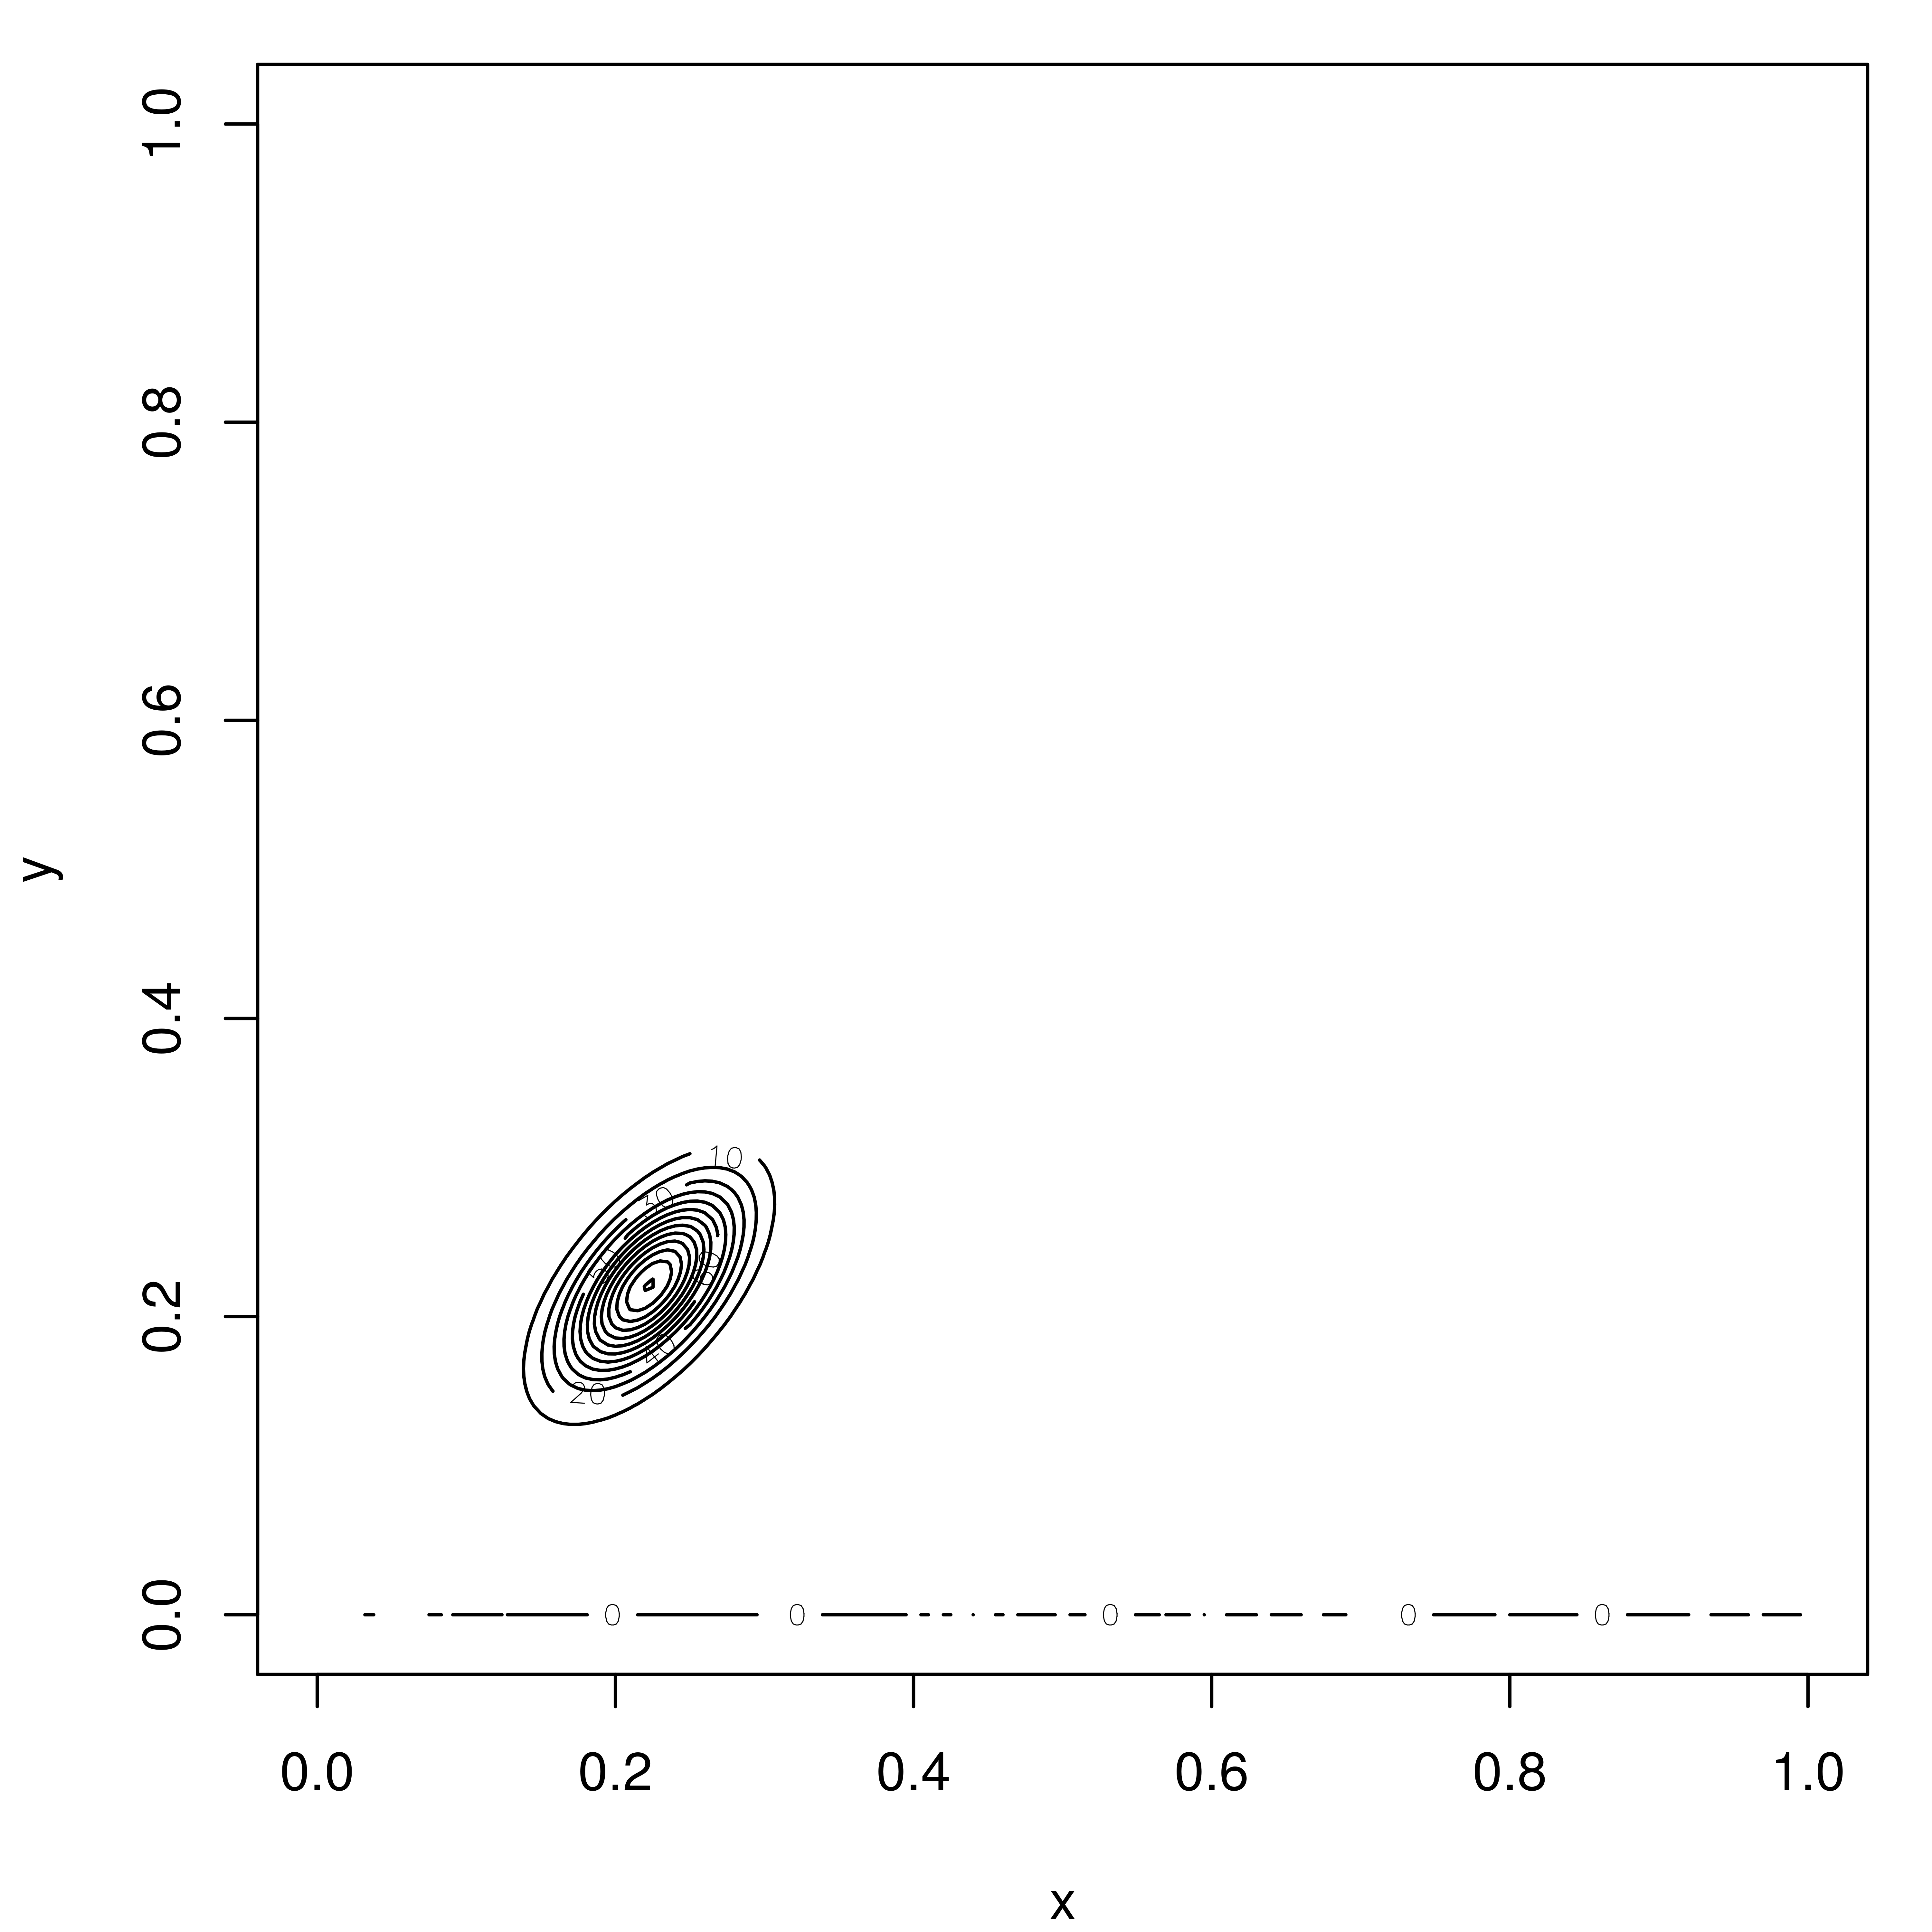
\includegraphics[width=1\linewidth]{../small-time-solution-contour.png}
    \end{minipage}
    %%
    & \begin{minipage}{0.3\textwidth}
      \centering
      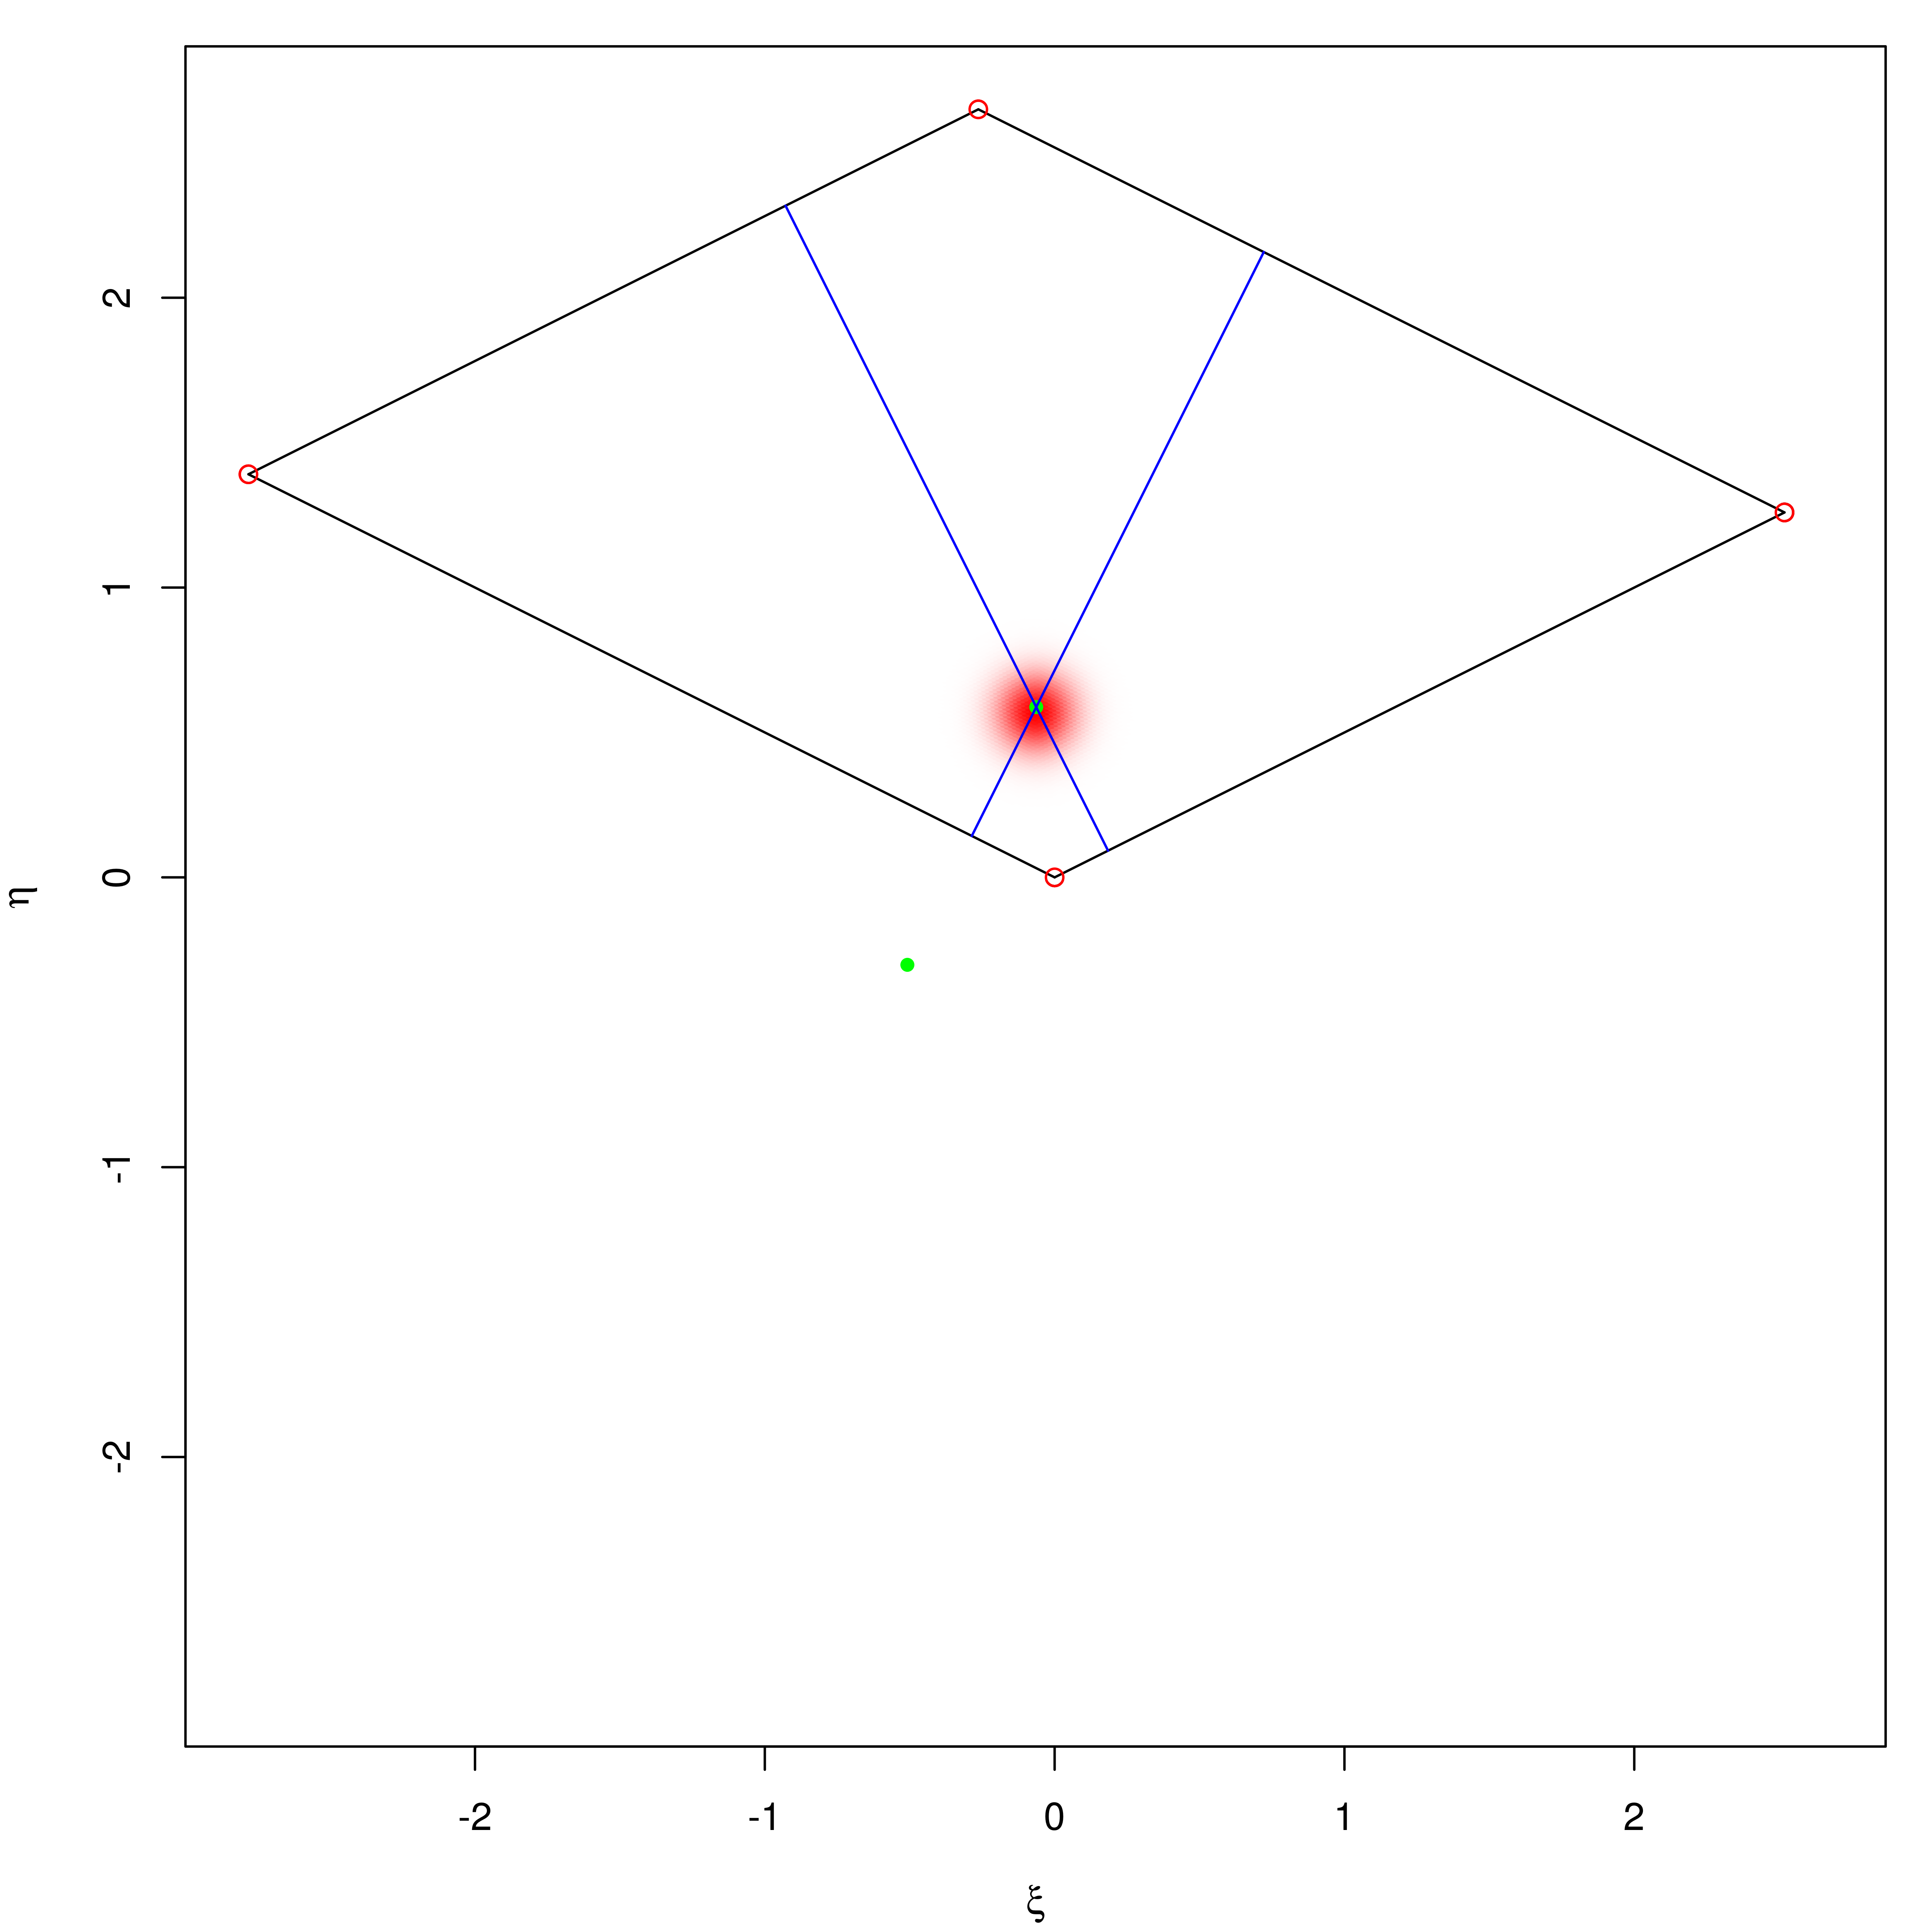
\includegraphics[width=1\linewidth]{../small-time-solution.png}
    \end{minipage}
  \end{tabular}
  %%
  %%
\end{figure}
\end{itemize}
\end{frame}
% ------------------------------------------------
\begin{frame}
  \frametitle{Consistency Results}
  Denoting the approximate density due to the Galerkin solution as
  \[
    f^{(k)}(x,y,a_x,b_x,a_y,b_y) = \frac{\partial^4
      q^{(k)}(x,y,t)}{\partial a_x \partial b_x \partial a_y \partial
      b_y},
  \]
  we show that the two integrals below converge in $L_2(\Omega)$:
  \begin{lemma}[1]\label{lem:1}
  \begin{multline*}
    \lim_{k\to \infty} \displaystyle \int_{a_x}^{b_x} \displaystyle
    \int_{a_y}^{b_y} f^{(k)}(x,y,a_x,b_x,a_y,b_y)\, dx\,dy = \\
    \displaystyle \int_{a_x}^{b_x} \displaystyle \int_{a_y}^{b_y}
    f(x,y,a_x,b_x,a_y,b_y)\, dx\,dy
  \end{multline*}
\end{lemma}
\end{frame}
% ------------------------------------------------
\begin{frame}
Denoting the random variable
\[Z := (X(t), Y(t), m_X(t), M_X(t), m_Y(t), M_Y(t)),\] we consider the
distribution function $F(Z \leq z)$ generated by the true solution to the
Fokker-Planck equation as well as the distribution $F^{(k)}(Z \leq z)$
generated by the Galerkin solution.
\begin{lemma}[Convergence in distribution] \label{lem:conv-dist}
  For any $z \in Z$,
  $ \lim_{k \to \infty} F^{(k)}(Z \leq z ) = F(Z \leq z).$
\end{lemma}

Assuming that the maximum likelihood estimate (MLE) (under $F^{(k)}$
for sufficiently large $k$) is continuous with respect to the data, we
can use the convergence result above and Chebyshev's inequality to
show that the MLE under $F^{(k)}$ is consistent as the number of basis
elements $k$ and number of data points $n$ go to infinity.
\end{frame}
% ------------------------------------------------
\begin{frame}
  \frametitle{Results and solution behavior for small $\tilde{t}$}
  \begin{figure}
  \centering
  \includegraphics[scale=0.5]{../chapter-2/figures/{limitations-rho-0.95-data-point-4}.pdf}
\end{figure}
The behavior of Galerkin solution is valid only up to a some small time $\tilde{t}$.
\end{frame}
% ------------------------------------------------
\begin{frame}
  \frametitle{Simulation Study} We consider $50$ simulated data sets with
  \begin{align*}
    \sigma_x &= 1, & \sigma_y &= 1, & \mu_x &= 0, & \mu_y &= 0
  \end{align*}
  with increasing sample size over several values of $\rho$. For each
  case, we consider the ratio of mean-square error of the Galerkin
  solver compared to that generated by Gaussian likelihoods ignoring the boundaries:
  \begin{table}  
  \centering
  \begin{tabular}{cccc|ccc}
    &  \multicolumn{3}{c}{$\rho=0.95$} & \multicolumn{3}{c}{$\rho=0.60$} \\
    & $m=4$ & $m=8$ & $m=16$ & $m=4$ & $m=8$ & $m=16$ \\
    \hline
    $\hat{\sigma}_x$ & 0.475 & 1.238 & 1.304 & 0.203 & 0.127 & 0.232   \\
    \hline
    $\hat{\sigma}_y$ & 0.593 & 1.040 & 1.088 &  0.111 & 0.120 & 0.260 \\
    \hline
    $\hat{\rho}$ & 0.287 & 0.910 & 0.445 & 0.315 & 0.283 & 0.463 
  \end{tabular}
\end{table}

  \begin{table}  
  \centering
  \begin{tabular}{cccc}
    & \multicolumn{3}{c}{$\rho=0.0$}\\
    & $m=4$ & $m=8$ & $m=16$ \\
    \hline
    $\hat{\sigma}_x$ & .137 & 0.243 & 0.167 \\
    \hline
    $\hat{\sigma}_y$ &  0.189 & 0.171 & 0.107 \\
    \hline
    $\hat{\rho}$ &  0.517 & 0.365 & 0.194
  \end{tabular}
  \end{table}

\end{frame}
% ------------------------------------------------
\begin{frame}
  \frametitle{Need for resolving the transient region}

  \begin{figure}
  \centering
  %%
  %%
  \begin{tabular}{ccc}
    
    \begin{minipage}{0.3\textwidth}
      \centering
      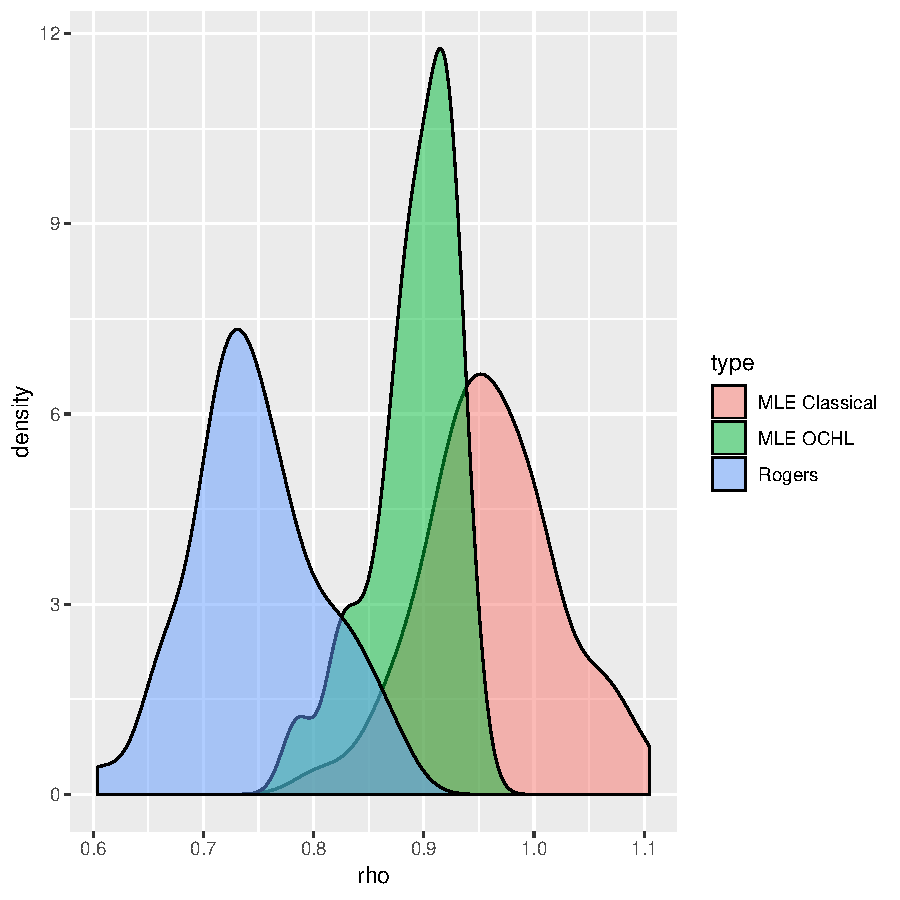
\includegraphics[width=1\linewidth]{../chapter-2/results/mle-results-rho-0.95-n-16/estimates-rho.pdf}
    \end{minipage}
    & \begin{minipage}{0.3\textwidth}
      \centering
      \includegraphics[width=1\linewidth]{../chapter-2/results/mle-results-rho-0.95-n-16/estimates-sigma-x.pdf}
    \end{minipage}
    & \begin{minipage}{0.3\textwidth}
      \centering
      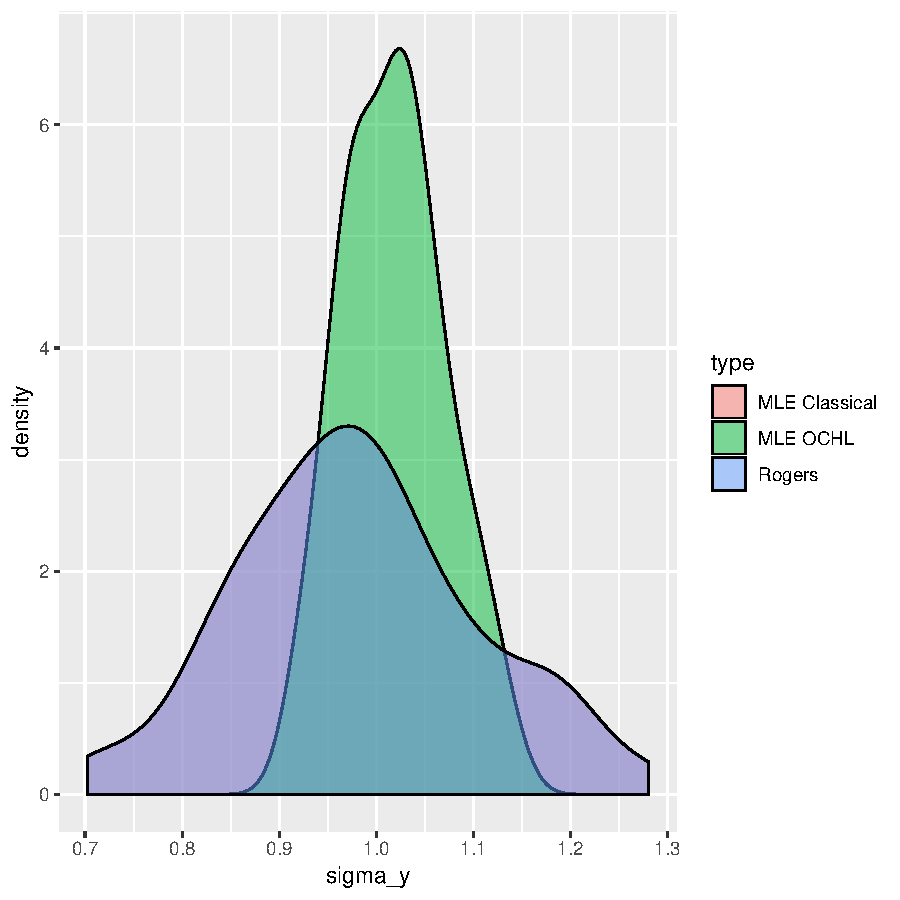
\includegraphics[width=1\linewidth]{../chapter-2/results/mle-results-rho-0.95-n-16/estimates-sigma-y.pdf}
    \end{minipage}
  \end{tabular}
  \caption{Data generated with $\rho=0.95$. Kernel-density
    approximations of the repeated-sampling densities of the MLEs are
    shown.  Samples are obtained from the Galerkin likelihood (green)
    and the classical likelihood (red) and the Rogers estimator
    (blue). The data-generating parameters are denoted with the
    vertical solid line.}
  \label{fig:mle-comparison-rho-0.95}
\end{figure}
  
\end{frame}


%------------------------------------------------
%------------------------------------------------
\section{Open, Close, High, Low Prices: Small Time Solution}
% ------------------------------------------------
\begin{frame}
Open, Close, High, Low Prices: Small Time Solution and Matching
\end{frame}
\begin{frame}
  \frametitle{Counterexample: method of images and analytic differentiability}
  \centering
  \includegraphics[scale=0.45]{../chapter-3/figures/chapter-3-figure-illustration-1.pdf}
\end{frame}
% ------------------------------------------------
\begin{frame}
  \frametitle{Symmetry constraint in constructing approximate solutions}

  A condition weaker than uniqueness which nonetheless restricts the
solution space is the symmetry obeyed by the problem. We consider the transformation
\begin{align*}
  x^{new} = (a_x + b_x) - x^{old}, \\
  y^{new} = (a_y + b_y) - y^{old}.
\end{align*}

Performing the set of reflections
\begin{align*}
  \left\{ 2,4,1,3 \right\} \cup \left\{ 2,4,3,1 \right\} \cup \left\{ 4,2,1,3 \right\} \cup \left\{ 4,2,3,1 \right\}. 
\end{align*}
produces a sum of images where only four elements are differentiable
with respecto to all four boundaries:

\[
  \frac{\partial^4 p_\epsilon(\tilde{x}, \tilde{y}, \tilde{t})}{\partial a_x \partial b_x \partial a_y \partial b_y}  = \sum_{j'=1}^{4}
                                                                                                                        \frac{\partial^4G(\tilde{x},\tilde{y},\tilde{t}|\tilde{x}_{(j')},\tilde{y}_{(j')})}{\partial a_x \partial b_x \partial a_y \partial b_y}.
\]

\end{frame}
% ------------------------------------------------
\begin{frame}
  \frametitle{Calculation of the joint density}
  We can express the derivatives:
\begin{align*}
  % \frac{\partial}{\partial a_x} G(x,y|t^{*}, \tilde{\sigma}, \rho, x_0^{(j^*)}, y_0^{(j^*)}) &= G \cdot \mathcal{C}\,\,\cdot \left( \frac{\partial \mathcal{P}}{\partial a_x} \right)\\
  % \frac{\partial^2}{\partial a_x \partial b_x} G(x,y|t^{*}, \tilde{\sigma}, \rho, x_0^{(j^*)}, y_0^{(j^*)}) &= G \cdot \mathcal{C}^2 \left( \frac{\partial \mathcal{P}}{\partial b_x} \right) \left( \frac{\partial \mathcal{P}}{\partial a_x} \right) + G \cdot \mathcal{C} \cdot \left( \frac{\partial^2 \mathcal{P}}{\partial a_x \partial b_x} \right) \\
  % %% %% %%
  % \frac{\partial^3}{\partial a_x \partial b_x \partial a_y} G(x,y|t^{*}, \tilde{\sigma}, \rho, x_0^{(j^*)}, y_0^{(j^*)}) &= G \cdot \mathcal{C}^3 \left( \frac{\partial \mathcal{P}}{\partial b_x} \right) \left( \frac{\partial \mathcal{P}}{\partial a_x} \right) \left( \frac{\partial \mathcal{P}}{\partial a_y} \right) \nonumber \\
  %                                                                                            &\,\, + G \cdot \mathcal{C}^2 \left[\left( \frac{\partial^2 \mathcal{P}}{\partial a_x \partial a_y} \right) \left( \frac{\partial \mathcal{P}}{\partial b_x} \right) + \left( \frac{\partial^2 \mathcal{P}}{\partial b_x \partial a_y} \right) \left( \frac{\partial \mathcal{P}}{\partial a_x} \right) + \left( \frac{\partial^2 \mathcal{P}}{\partial a_x \partial b_x} \right) \left( \frac{\partial \mathcal{P}}{\partial a_y} \right)\right] \nonumber \\
  %                                                                                            &\,\, + G \cdot \mathcal{C} \left( \frac{\partial^3 \mathcal{P}}{\partial a_x \partial b_x \partial a_y} \right) \nonumber \\
  %                                                                                            %% %% %%
  \frac{\partial^4}{\partial a_x \partial b_x \partial a_y \partial b_y} G(\tilde{x},\tilde{y},\tilde{t} |  \tilde{x}_{(j)}, \tilde{y}_{(j)}) &= \\
  \MoveEqLeft[15] G \cdot \mathcal{C}^4 \cdot \left(\partial_{a_x}\partial_{b_x} \partial_{a_y}\partial_{b_y} \right)\mathcal{P}&  \nonumber \\
  \MoveEqLeft[15] \,\, + G \cdot \mathcal{C}^3 \cdot \left( \partial^2_{a_x\, b_x} \partial_{a_y} \partial_{b_y} + \partial^2_{a_x\, a_y} \partial_{b_x} \partial_{b_y} + \partial^2_{a_x\, b_y} \partial_{b_x} \partial_{a_y} + \right. &\nonumber \\
  \MoveEqLeft[15] \left. \qquad\qquad\qquad +\partial^2_{b_x\, a_y} \partial_{a_x} \partial_{b_y} + \partial^2_{b_x\, b_y} \partial_{a_x} \partial_{a_y} \partial^2_{a_y\, b_y} \partial_{a_x} \partial_{b_x} \right) \mathcal{P} &  \nonumber \\
  \MoveEqLeft[15] \,\, + G \cdot \mathcal{C}^2 \cdot \left( \partial^3_{a_x\,b_x\,a_y} \partial_{b_y} + \partial^2_{a_x\,b_x}\partial^2_{a_y\,b_y} + \partial^3_{a_x\,b_x\,b_y}\partial_{a_y}  + \right.& \nonumber \\
  \MoveEqLeft[15] \left. \qquad\qquad\qquad + \partial^3_{a_x\,a_y\,b_y} \partial_{b_x} + \partial^2_{a_x\,a_y} \partial^2_{b_y\,b_x} + \partial^3_{b_x\,a_y\,b_y}\partial_{a_x} + \partial^2_{b_x\,a_y}\partial_{a_x}\partial_{b_y} \right) \mathcal{P} & \nonumber \\
  \MoveEqLeft[15] \,\, + G \cdot \mathcal{C} \cdot \partial^4_{a_x\,b_x\,a_y\,b_y} P,& \label{eq:fourth-deriv}
\end{align*}
\end{frame}
% ------------------------------------------------
\begin{frame}
  \frametitle{Analytic Derivative and higher order terms}

  Thinking of $\tilde{t}$ as variable allows us to further simplify
  the expression. Since $\mathcal{C} = \mathcal{O}(1/\tilde{t})$, all
  three terms $G\cdot \mathcal{C}^3, G\cdot \mathcal{C}^2,$ and
  $G\cdot \mathcal{C}$ are
  $o\left( G\cdot \mathcal{C}^4 \cdot
    \left(\partial_{a_x}\partial_{b_x} \partial_{a_y}\partial_{b_y}
    \right)\mathcal{P} \right)$, so that the $G\cdot \mathcal{C}^4$
  order term in the derivative dominates the others for sufficiently
  small $\,\,\tilde{t}$.

  \begin{align*}
  \frac{\partial^4 p_\epsilon(\tilde{x}, \tilde{y}, \tilde{t})}{\partial a_x
  \partial b_x \partial a_y \partial b_y} &\approx \sum_{j'=1}^{4} G(\tilde{x},\tilde{y},\tilde{t}|\tilde{x}_{(j')},\tilde{y}_{(j')}) \cdot \mathcal{C}^4 \cdot \left(\partial_{a_x}\partial_{b_x} \partial_{a_y}\partial_{b_y} \right)\mathcal{P}_{j'}. 
\end{align*}
\end{frame}
% ------------------------------------------------
\begin{frame}
  \frametitle{Illustration of proof for existence}
\end{frame}
% ------------------------------------------------
\begin{frame}
  \frametitle{Basis Expansion of Galerkin likelihood: RHS}
  The likelihood computed with the Galerkin solution as a
function of $\tilde{t}$ is of the form
\begin{align*}
  \frac{\partial^4 p_{G}(\tilde{x}, \tilde{y}, \tilde{t})}{\partial a_x
  \partial b_x \partial a_y \partial b_y} = \sum_{k=1}^{K} e^{-\lambda_k\tilde{t}} p_k^{(4)}(\tilde{t}),
\end{align*}
where $p_i^{(4)}(\tilde{t})$ is a fourth-order polynomial. This
proceeds from the Galerkin solution being dependent on $\tilde{t}$
only through the exponential term: the eigenfunctions of the solution
are by design solely functions of $(a_x, b_x, a_y, b_y)$ and
$(\tilde{x}, \tilde{y})$


\begin{itemize}
\item This suggests a leading-order approximation that is fitted with the Galerking solver via least squares:
  \begin{align*}
    f_{LS}(\tilde{t}) &= \tilde{t}^4 \left( \omega_1 e^{-\lambda_1\tilde{t}} + \omega_2 e^{-\lambda_2\tilde{t}}\right).
  \end{align*}
\end{itemize}
\end{frame}
% ------------------------------------------------
\begin{frame}
  \frametitle{Leading order for small-time solution: LHS}

  The summand in the small-time likelihood with the greatest
  $\beta_{j'}$ contributes the most to the truncated small-time
  solution in the $\tilde{t} \leq 1$ region where the matched solution
  will be applied. Indexing $j'$ such that
  $\beta_1 \geq \beta_2 \geq \beta_3 \geq \beta_4$, the small-time
  log-likelihood is
\begin{align*}
  \log\left( \frac{\partial^4 p_\epsilon(\tilde{x}, \tilde{y}, \tilde{t})}{\partial a_x
  \partial b_x \partial a_y \partial b_y} \right) &\approx \log(K) - 4.5\log(\tilde{t}) + \log(c_1) - \frac{\beta_1}{\tilde{t}} \nonumber \\
  &\quad + \log\left(1 + \sum_{j \neq 1} \frac{c_j}{c_1}\exp\left( -\frac{(\beta_j-\beta_1)}{\tilde{t}} \right) \right) \nonumber \\
  &\approx \log(K) - 4.5\log(\tilde{t}) + \log(c_1) - \frac{\beta_1}{\tilde{t}} + \log\left(1 + \epsilon(\tilde{t}) \right), 
\end{align*}

  \begin{itemize}
\item The proposed matched solution is of the form
  \[
    \log f_{\mbox{matched}}(\tilde{t}) = \log(\omega(\tilde{t})) -
    \gamma(\tilde{t})\log(\tilde{t}) -
    \frac{\beta(\tilde{t})}{\tilde{t}}
  \]
  \end{itemize}
\end{frame}
% ------------------------------------------------
\begin{frame}
At $\tilde{t}^*$, the
left-hand side of the matching condition, the values for these
parameters are defined such that they match the small-time solution
\begin{align*}
  \omega(\tilde{t}^*) &= K, & \gamma(\tilde{t}^*) &= 4.5, & \beta(\tilde{t}^*) &= \beta_1.
\end{align*}
At $\tilde{t}_m$, the right-hand side of the matching condition and
the maximum of the LS solution,
$\omega(\tilde{t}), \gamma(\tilde{t}),$ and $\beta(\tilde{t})$ are
chosen to match the value, first, and second derivatives of the
logarithmic form of the LS solution. The form of the parameters
between $\tilde{t}^*$ and $\tilde{t}_m$ is chosen to be a sigmoid
function which rapidly transitions away from $\tilde{t}^*$ and is the
same for all three parameters:
\begin{align*}
    \omega(\tilde{t}) &= \omega(\tilde{t}^*)e^{-k(\tilde{t}-\tilde{t}^*)} + \omega(\tilde{t}_m)\left(1-e^{-k(\tilde{t}-\tilde{t}^*)}\right), \\
    \gamma(\tilde{t}) &= \gamma(\tilde{t}^*)e^{-k(\tilde{t}-\tilde{t}^*)} + \gamma(\tilde{t}_m)\left(1-e^{-k(\tilde{t}-\tilde{t}^*)}\right), \\
    \beta(\tilde{t}) &= \beta(\tilde{t}^*)e^{-k(\tilde{t}-\tilde{t}^*)} + \beta(\tilde{t}_m)\left(1-e^{-k(\tilde{t}-\tilde{t}^*)}\right).
\end{align*}
\end{frame}
% ------------------------------------------------
\begin{frame}
  \centering
  \includegraphics[scale=0.8]{../chapter-3/figures/{matched-rho-0.95-data-point-4}.pdf}
\end{frame}
% ------------------------------------------------
\begin{frame}
  \frametitle{Repeated Simulation Results}
  \begin{table}
  \centering
  \begin{tabular}{cccc}
    \multicolumn{4}{c}{$\rho=0.95$} \\
    & $m=4$ & $m=8$ & $m=16$ \\
    \hline
    $\hat{\sigma}_x$ & 0.124 & 0.429  & 0.318 \\
    \hline
    $\hat{\sigma}_y$ & 0.310 & 0.147  & 0.365 \\
    \hline
    $\hat{\rho}$ & 0.250 & 0.753 & 0.699
  \end{tabular}
\end{table}
\end{frame}

\begin{frame}
\centering
\includegraphics[scale=0.5]{../chapter-3/results/mle-results-rho-0.95-n-16/estimates-sigma-x.pdf}
\end{frame}

\begin{frame}
  \frametitle{Future work}
\end{frame}

\end{document} 


